\documentclass[12pt,a4paper]{article}
\title{MATH1106 DIS207/208 Practice Quiz 2}
\author{Benjamin Thompson}
\date{February 26, 2020}

\usepackage[margin=1in]{geometry}

\usepackage{amsmath}
\usepackage[usenames,dvipsnames]{xcolor}
\usepackage{tikz}
\usetikzlibrary{arrows.meta,decorations.markings}


\usepackage{pgfplots}

\pgfplotsset{every axis/.append style={
axis x line=middle,    % put the x axis in the middle
axis y line=middle,    % put the y axis in the middle
axis line style={-{Stealth[length=3mm]},color=black}, % arrows on the axis
minor tick num=1
            }}


\usepackage{fancyhdr}
\pagestyle{fancy}

\fancyhf{}
\lhead{MATH1106 DIS207/208 Practice Quiz 2}
\rhead{February 26, 2020}
\cfoot{\thepage}

\usepackage{enumitem}

\newcommand{\bfa}{\mathbf{a}}
\newcommand{\bfb}{\mathbf{b}}
\newcommand{\bfc}{\mathbf{c}}
\newcommand{\bfd}{\mathbf{d}}


\begin{document}
\subsubsection*{Name:}
Each of the multiple choice questions below has one correct choice. Circle the correct choice. (NOTE: The quiz presented in class had errors in Q1 and Q2, these have been corrected.)
\subsubsection*{Q1}
An SIR model of an epidemic is created and described by the following differential equations, where $A$, $B$, $C$ represent susceptible, infectious, and recovered populations, but not necessarily in that order.
\begin{align*}
A' &= \gamma C \\
B' &= -\beta BC  \\
C' &= \beta BC - \gamma C
\end{align*}
A vaccine is developed, and the model is updated to incorporate this change. Assuming that vaccinated individuals are immune from the disease and are not infectious, which of the following is a change equation in the new model?

\begin{enumerate}[label=(\alph*)]
\item $A' = \gamma C - \delta A$
\item $B' = -\beta BC - \delta B$
\item $C' = \beta BC - \gamma A - \delta A$
\item $C' = \beta BC - \gamma A + \delta A$
\end{enumerate}

\subsubsection*{Q2}
Recall the Romeo and Juliet model given by the change equations
\begin{align*}
	J' &= R \\
	R' &= -J.
\end{align*}
Which of the following statements regarding the vector field of the model is false?
\begin{enumerate}[label=(\alph*)]
\item If the vector field is rotated by $180^{\circ}$ around the origin, the rotated vector field is identical to original vector field.
\item The length of a vector at a point $(A,A)$ is $|A|\sqrt{2}$.
\item Only one vector in the vector field has length $0$.
\item Vectors at different points have different directions.
\end{enumerate}

\subsubsection*{Q3}
The growth of a certain protozoa population is found to be described by
\[
	P' = \sqrt{P} + 4.
\]
At time $t=100$ the population is $9$. Euler's method is used to estimate the population at time $t=102$ using the interval $\Delta t = 1$. This estimate is:

\begin{enumerate}[label=(\alph*)]
\item $4 + \sqrt{7}$
\item $16$
\item $24$
\item $18 + \sqrt{14}$
\end{enumerate}

\subsubsection*{Q4}
A line in the $xy$-plane has passes through the points $(2,0)$ and $(0,1)$. The line has slope:
\begin{enumerate}[label=(\alph*)]
\item $-2$
\item $2$
\item $-\frac{1}{2}$
\item $\frac{1}{2}$
\end{enumerate}

\newpage

\subsubsection*{Q5}
The state space trajectory of a system with variables $M$, $N$ is shown below. Assuming that as time increases \emph{the trajectory goes in a clockwise direction}, which of the following graphs is a possible time-series of the trajectory? (Note: in the time-series graphs, the horizontal axis represents time.)
\[
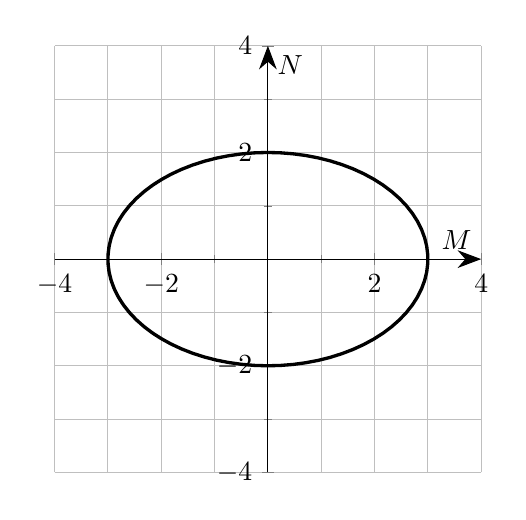
\begin{tikzpicture}
\begin{axis}[xlabel={$M$},ylabel={$N$},width=7cm, height=7cm, xmin=-4,xmax=4, ymin=-4,ymax=4, grid=both]
\addplot [very thick, domain=-4:4,samples=100]({3*cos(deg(x))},{2*sin(deg(x))}); 
\end{axis}
\end{tikzpicture}
\]
\[
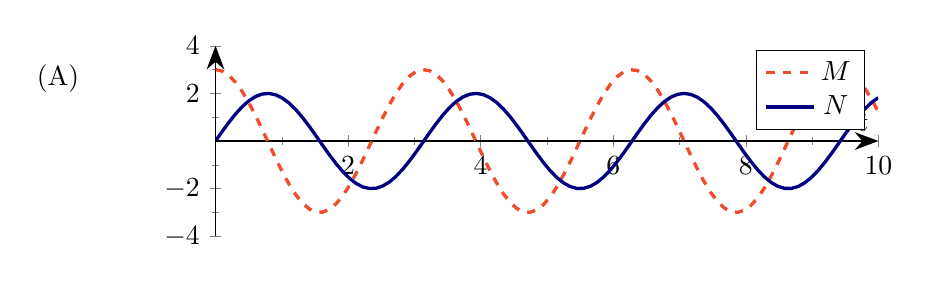
\begin{tikzpicture}

\begin{axis}[xlabel={$t$},width=10cm, height=4cm, xmin=0,xmax=10, ymin=-4,ymax=4, grid=none]
\addplot [dashed,RedOrange,very thick,domain=0:10,samples=100]{3*cos(2*deg(x))};
\addlegendentry{$M$}
\addplot [NavyBlue,very thick, domain=0:10,samples=100]{2*sin(2*deg(x))}; 
\addlegendentry{$N$}
\end{axis}

\node (A) at (-2,2) {(A)};
\end{tikzpicture}
\]
\[
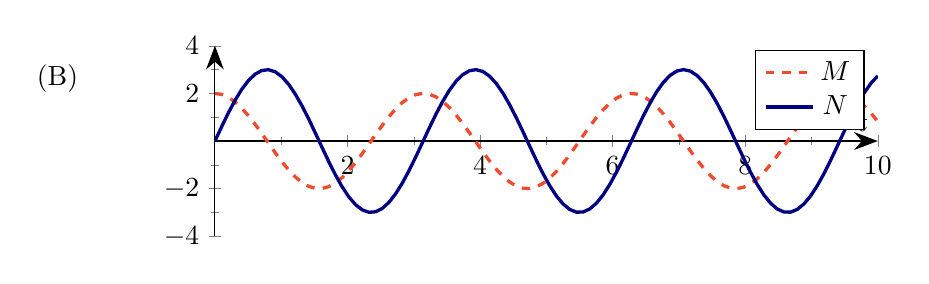
\begin{tikzpicture}

\begin{axis}[xlabel={$t$},width=10cm, height=4cm, xmin=0,xmax=10, ymin=-4,ymax=4, grid=none]
\addplot [dashed,RedOrange,very thick,domain=0:10,samples=100]{2*cos(2*deg(x))};
\addlegendentry{$M$}
\addplot [NavyBlue,very thick, domain=0:10,samples=100]{3*sin(2*deg(x))}; 
\addlegendentry{$N$}
\end{axis}

\node (B) at (-2,2) {(B)};
\end{tikzpicture}
\]
\[
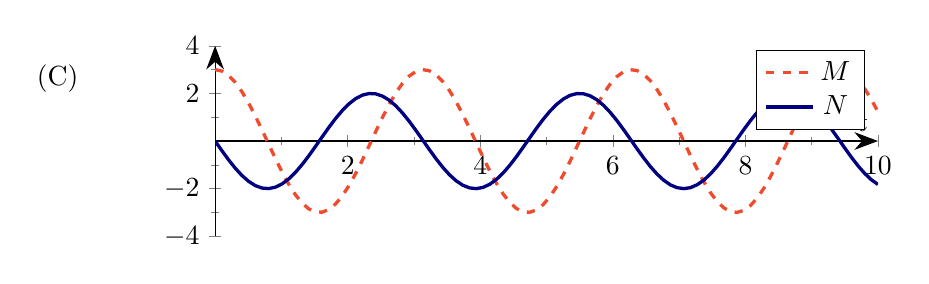
\begin{tikzpicture}

\begin{axis}[xlabel={$t$},width=10cm, height=4cm, xmin=0,xmax=10, ymin=-4,ymax=4, grid=none]
\addplot [dashed,RedOrange,very thick,domain=0:10,samples=100]{3*cos(2*deg(x))};
\addlegendentry{$M$}
\addplot [NavyBlue,very thick, domain=0:10,samples=100]{-2*sin(2*deg(x))}; 
\addlegendentry{$N$}
\end{axis}

\node (C) at (-2,2) {(C)};
\end{tikzpicture}
\]
\[
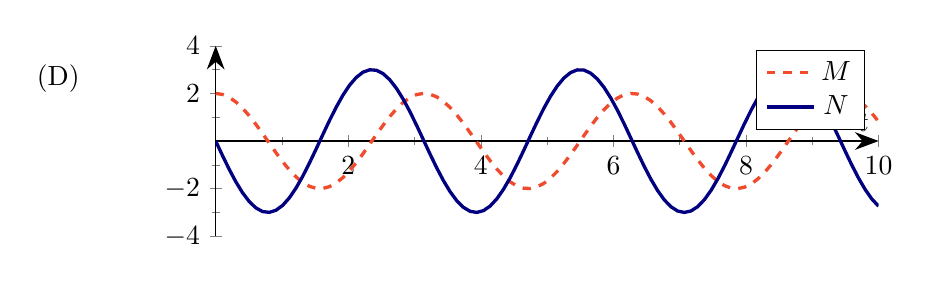
\begin{tikzpicture}

\begin{axis}[xlabel={$t$},width=10cm, height=4cm, xmin=0,xmax=10, ymin=-4,ymax=4, grid=none]
\addplot [dashed, RedOrange,very thick,domain=0:10,samples=100]{2*cos(2*deg(x))};
\addlegendentry{$M$}
\addplot [NavyBlue,very thick, domain=0:10,samples=100]{-3*sin(2*deg(x))}; 
\addlegendentry{$N$}
\end{axis}

\node (D) at (-2,2) {(D)};
\end{tikzpicture}
\]

\end{document}
